\chapter{LaTeX使用说明}\label{chap:guide}

{
为方便使用及更好地展示LaTeX排版的优秀特性,ucasthesis的框架和文件体系进行了细致地处理,尽可能地对各个功能和板块进行了模块化和封装。zhkuThesis基于ucasthesis做了自定义的样式修改和整理说明。

\section{初步设置}

\begin{enumerate}
    \item 使用overleaf:打开并注册\href{https://cn.overleaf.com/}{overleaf}。
    \item 将整个文件夹上传至overleaf项目。
    \item 右键菜单,设置编译器为XeLaTeX,选择TexLive 2021
    \item 点击编译,即可预览PDF文件
\end{enumerate}

编译完成即可获得本PDF说明文档。

\section{文档目录简介}

\subsection{zhkuThesis.tex}

zhkuThesis.tex为主文档,其设计和规划了论文的整体框架,通过对其的阅读可以了解整个论文框架的搭建。

\subsection{编译脚本}

为方便本地编译,提供bat脚本和.sh脚本分别用于windows环境和unix环境。

\begin{itemize}
    \item Windows:双击Dos脚本artratex.bat可得全编译后的PDF文档,其存在是为了帮助不了解LaTeX编译过程的初学者跨过编译这第一道坎,请勿通过邮件传播和接收此脚本,以防范Dos脚本的潜在风险。
    \item Linux或MacOS:在terminal中运行
        \begin{itemize}
            \item \verb|./artratex.sh xa|:获得全编译后的PDF文档
            \item \verb|./artratex.sh x|:快速编译,不会生成文献引用
        \end{itemize}
\end{itemize}

全编译指运行 \verb|xeLaTeX+bibtex+xeLaTeX+xeLaTeX| 以正确生成所有的引用链接,如目录、参考文献及引用等。在写作过程中若无添加新的引用,则可用快速编译,即只运行一遍LaTeX编译引擎以减少编译时间。

\subsection{Tmp文件夹}

运行编译脚本后,编译所生成的文档皆存于Tmp文件夹内,包括编译得到的PDF文档,其存在是为了保持工作空间的整洁。

\subsection{Style文件夹}

包含zhkuThesis文档类的定义文件和配置文件,通过对它们的修改可以实现特定的模版设定。

\begin{enumerate}
    \item zhkuThesis.cls:文档类定义文件,论文的最核心的格式即通过它来定义的。
    \item zhkuThesis.cfg:文档类配置文件,设定如目录显示为“目~录”而非“目录”。
    \item artratex.sty: 常用宏包及文档设定,如参考文献样式、文献引用样式、页眉页脚设定等。这些功能具有开关选项,常只需在Thesis.tex中进行启用即可,一般无需修改artratex.sty本身。
    \item artracom.sty:自定义命令以及添加宏包的推荐放置位置。
\end{enumerate}

\subsection{Tex文件夹}

文件夹内为论文的所有实体内容,正常情况下,这也是使用zhkuThesis撰写学位论文时,主要关注和修改的一个位置,注:所有文件都必须采用UTF-8编码,否则编译后将出现乱码文本,详细分类介绍如下:

\begin{itemize}
    \item Frontinfo.tex:为论文中英文封面信息。论文封面会根据英文学位名称如Master,Doctor自动切换为相应的格式。
    \item Frontmatter.tex:为论文前言内容如中英文摘要等。
    \item Mainmatter.tex:索引需要出现的Chapter。开始写论文时,可以只索引当前章节,以快速编译查看,当论文完成后,再对所有章节进行索引即可。
    \item Chap{\_}xxx.tex:为论文主体的各章,可根据需要添加和撰写。添加新章时,可拷贝一个已有的章文件再重命名,以继承文档的 UTF8 编码。
    \item Appendix.tex:为附录内容。
    \item Backmatter.tex:为发表文章信息和致谢部分等。
\end{itemize}

\subsection{Image文件夹}

用于放置论文中所需要的图类文件,支持格式有:.jpg, .png, .pdf。其中,\verb|zhku_logo.png|为仲恺农业工程学院校徽校名。

\subsection{Biblio文件夹}

 ref.bib用于放置论文中所需要参考文献信息。

\section{功能介绍}

\subsection{数学公式}

比如Navier-Stokes方程(方程~\eqref{eq:ns}):
\begin{equation} \label{eq:ns}
    %\adddotsbeforeeqnnum%
    \begin{cases}
        \frac{\partial \rho}{\partial t} + \nabla\cdot(\rho\Vector{V}) = 0 \ \mathrm{times\ math\ test: 1,2,3,4,5}, 1,2,3,4,5\\
        \frac{\partial (\rho\Vector{V})}{\partial t} + \nabla\cdot(\rho\Vector{V}\Vector{V}) = \nabla\cdot\Tensor{\sigma} \ \text{times text test: 1,2,3,4,5}\\
        \frac{\partial (\rho E)}{\partial t} + \nabla\cdot(\rho E\Vector{V}) = \nabla\cdot(k\nabla T) + \nabla\cdot(\Tensor{\sigma}\cdot\Vector{V})
    \end{cases}
\end{equation}
\begin{equation}
    %\adddotsbeforeeqnnum%
    \frac{\partial }{\partial t}\int\limits_{\Omega} u \, \mathrm{d}\Omega + \int\limits_{S} \unitVector{n}\cdot(u\Vector{V}) \, \mathrm{d}S = \dot{\phi}
\end{equation}
\[
    \begin{split}
        \mathcal{L} \{f\}(s) &= \int _{0^{-}}^{\infty} f(t) e^{-st} \, \mathrm{d}t, \ 
        \mathscr{L} \{f\}(s) = \int _{0^{-}}^{\infty} f(t) e^{-st} \, \mathrm{d}t\\
        \mathcal{F} {\bigl (} f(x+x_{0}) {\bigr )} &= \mathcal{F} {\bigl (} f(x) {\bigr )} e^{2\pi i\xi x_{0}}, \ 
        \mathscr{F} {\bigl (} f(x+x_{0}) {\bigr )} = \mathscr{F} {\bigl (} f(x) {\bigr )} e^{2\pi i\xi x_{0}}
    \end{split}
\]

数学公式常用命令请见 \href{https://en.wikibooks.org/wiki/LaTeX/Mathematics}{WiKibook Mathematics}。artracom.sty中对一些常用数据类型如矢量矩阵等进行了封装,这样的好处是如有一天需要修改矢量的显示形式,只需单独修改artracom.sty中的矢量定义即可实现全文档的修改。

\subsection{数学环境}

\begin{axiom}
   这是一个公理。 
\end{axiom}
\begin{theorem}
   这是一个定理。 
\end{theorem}
\begin{lemma}
   这是一个引理。 
\end{lemma}
\begin{corollary}
   这是一个推论。 
\end{corollary}
\begin{assertion}
   这是一个断言。 
\end{assertion}
\begin{proposition}
   这是一个命题。 
\end{proposition}
\begin{definition}
    这是一个定义。
\end{definition}
\begin{example}
    这是一个例子。
\end{example}
\begin{remark}
    这是一个注。
\end{remark}

\subsection{图}

论文中图片的插入通常分为单图和多图,下面分别加以介绍:

单图插入:假设插入名为\verb|c06h06|(后缀可以为.jpg、.png和.pdf,下同)的图片,其效果如图~\ref{fig:c06h06}。
\begin{figure}[!htbp]
    \centering
    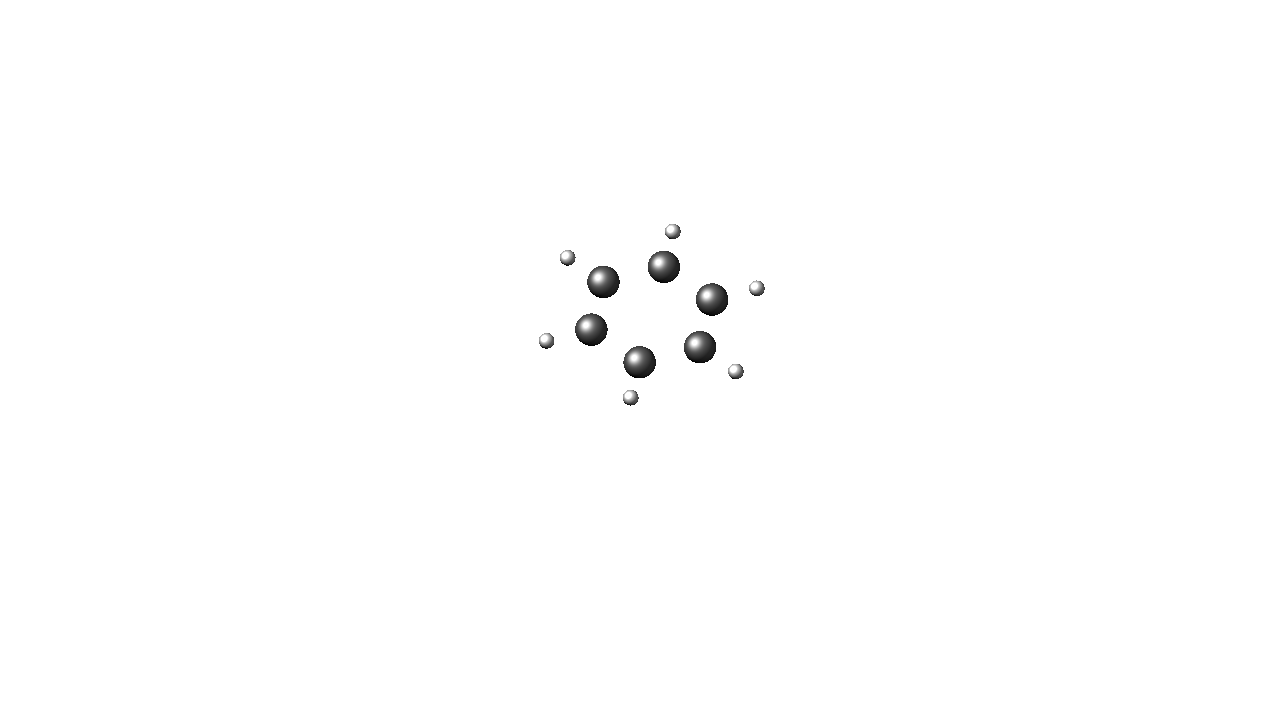
\includegraphics[width=0.40\textwidth]{c06h06}
    \bicaption{\quad 样图}{\quad Sample Figure}
    \label{fig:c06h06}
\end{figure}

如果插图的空白区域过大,以图片\verb|c06h06|为例,自动裁剪如图~\ref{fig:c06h06_trim}。
\begin{figure}[!htbp]
    \centering
    %trim option's parameter order: left bottom right top
    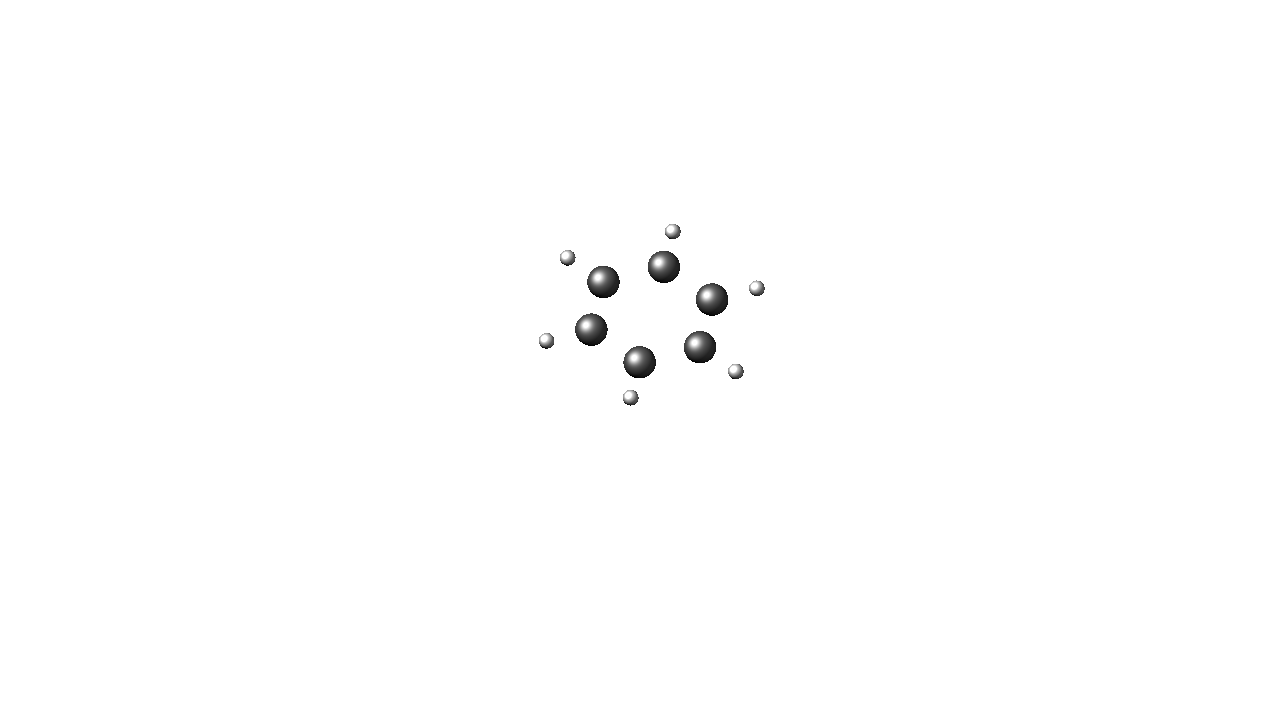
\includegraphics[trim = 60mm 80mm 60mm 60mm, clip, width=0.40\textwidth]{c06h06}
    \bicaption{\quad 自动裁切测试}{\quad Auto-Crop Test}
    \label{fig:c06h06_trim}
\end{figure}

多图的插入如图~\ref{fig:oaspl},多图不应在子图中给文本子标题,只要给序号,并在主标题中进行引用说明。
\begin{figure}[!htbp]
    \centering
    \begin{subfigure}[b]{0.35\textwidth}
      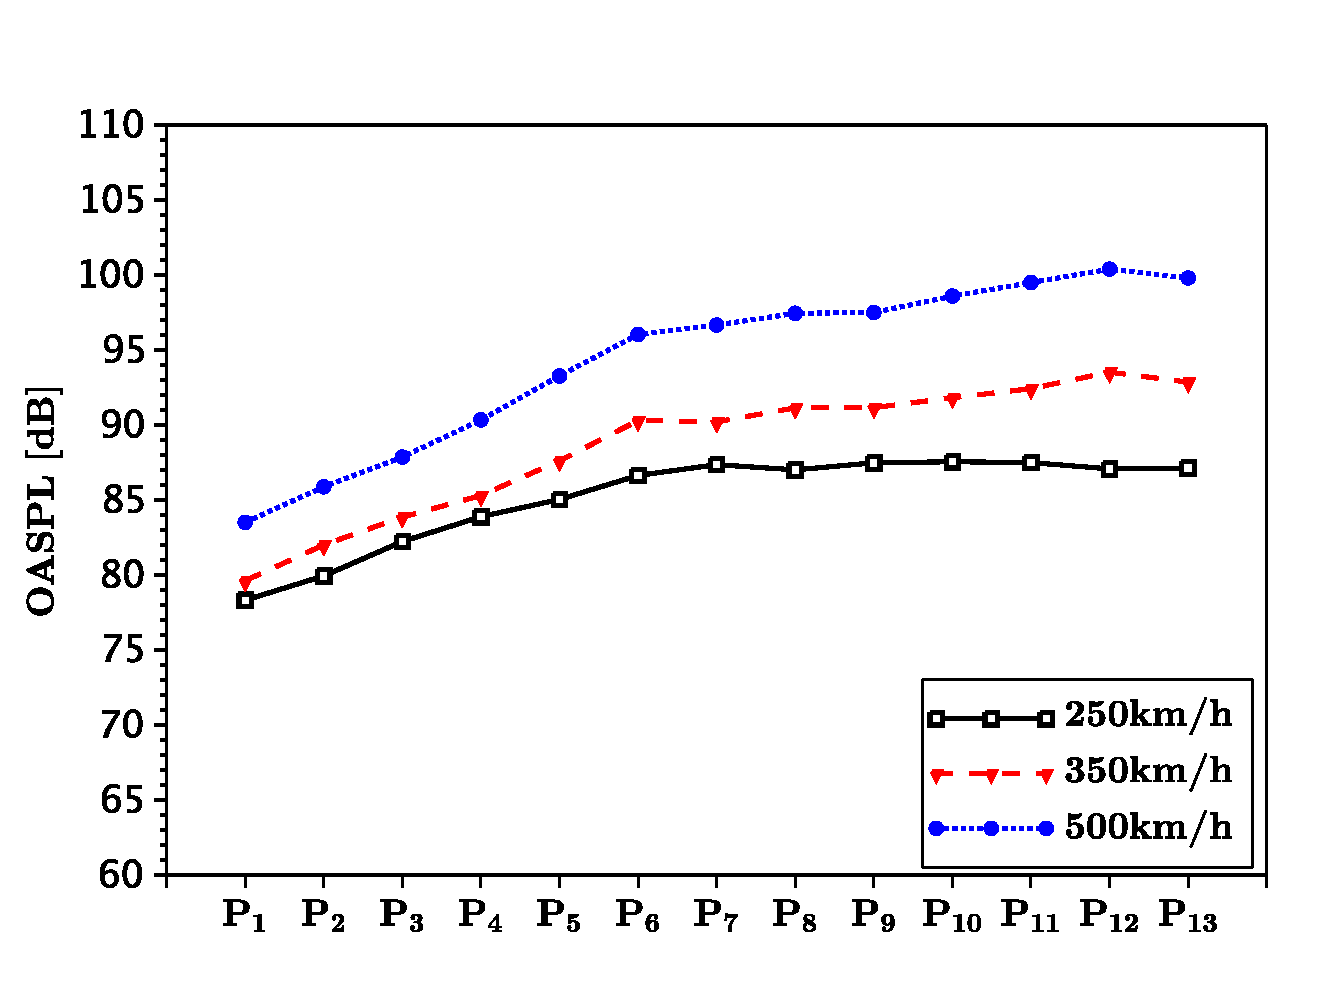
\includegraphics[width=\textwidth]{oaspl_a}
      \caption{}
      \label{fig:oaspl_a}
    \end{subfigure}%
    ~% add desired spacing
    \begin{subfigure}[b]{0.35\textwidth}
      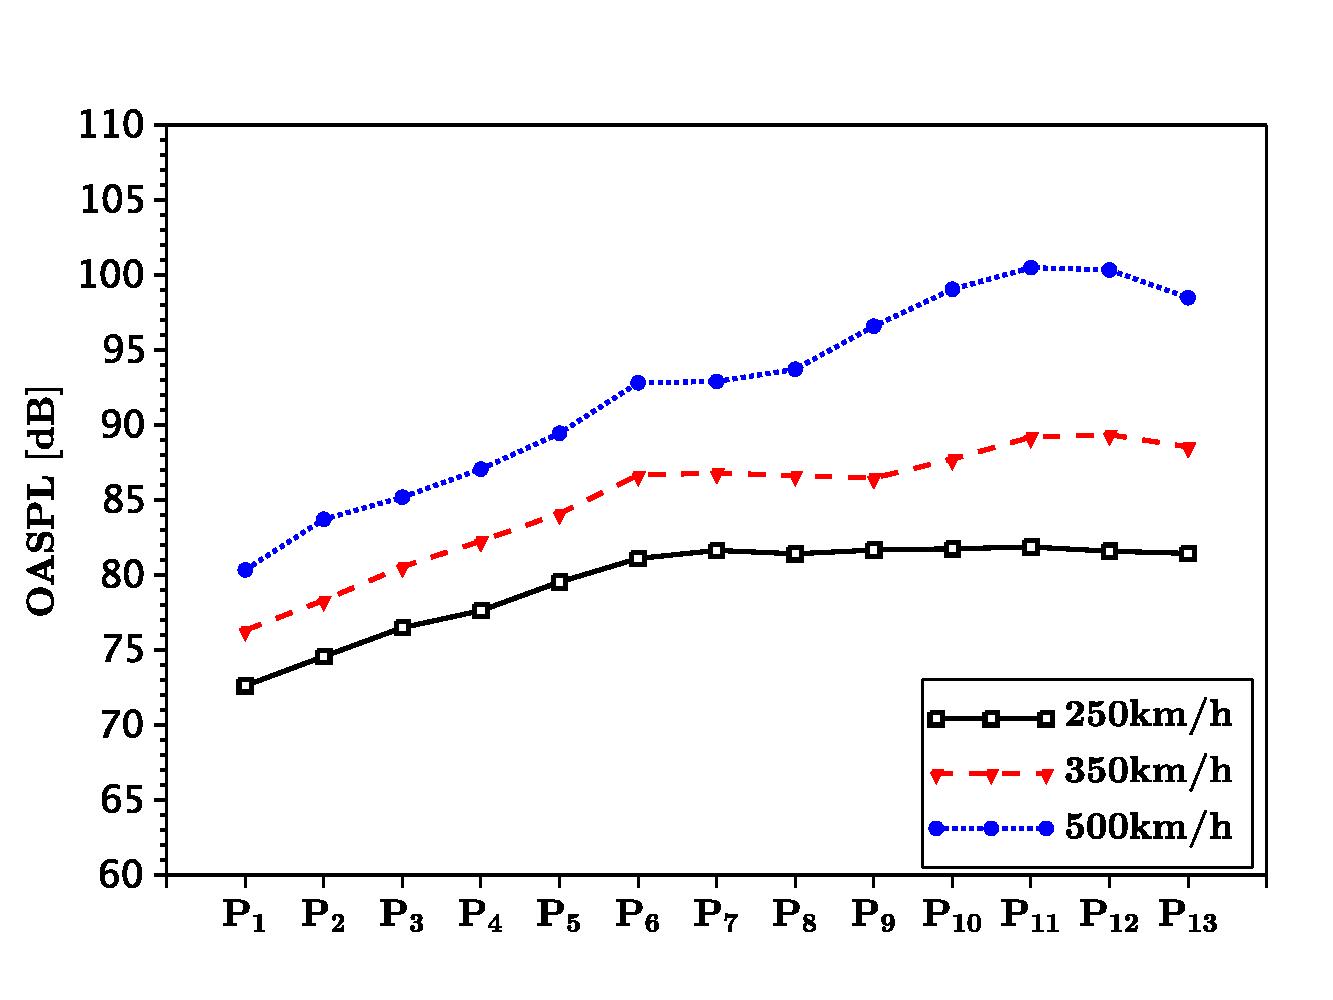
\includegraphics[width=\textwidth]{oaspl_b}
      \caption{}
      \label{fig:oaspl_b}
    \end{subfigure}
    \\% line break
    \begin{subfigure}[b]{0.35\textwidth}
      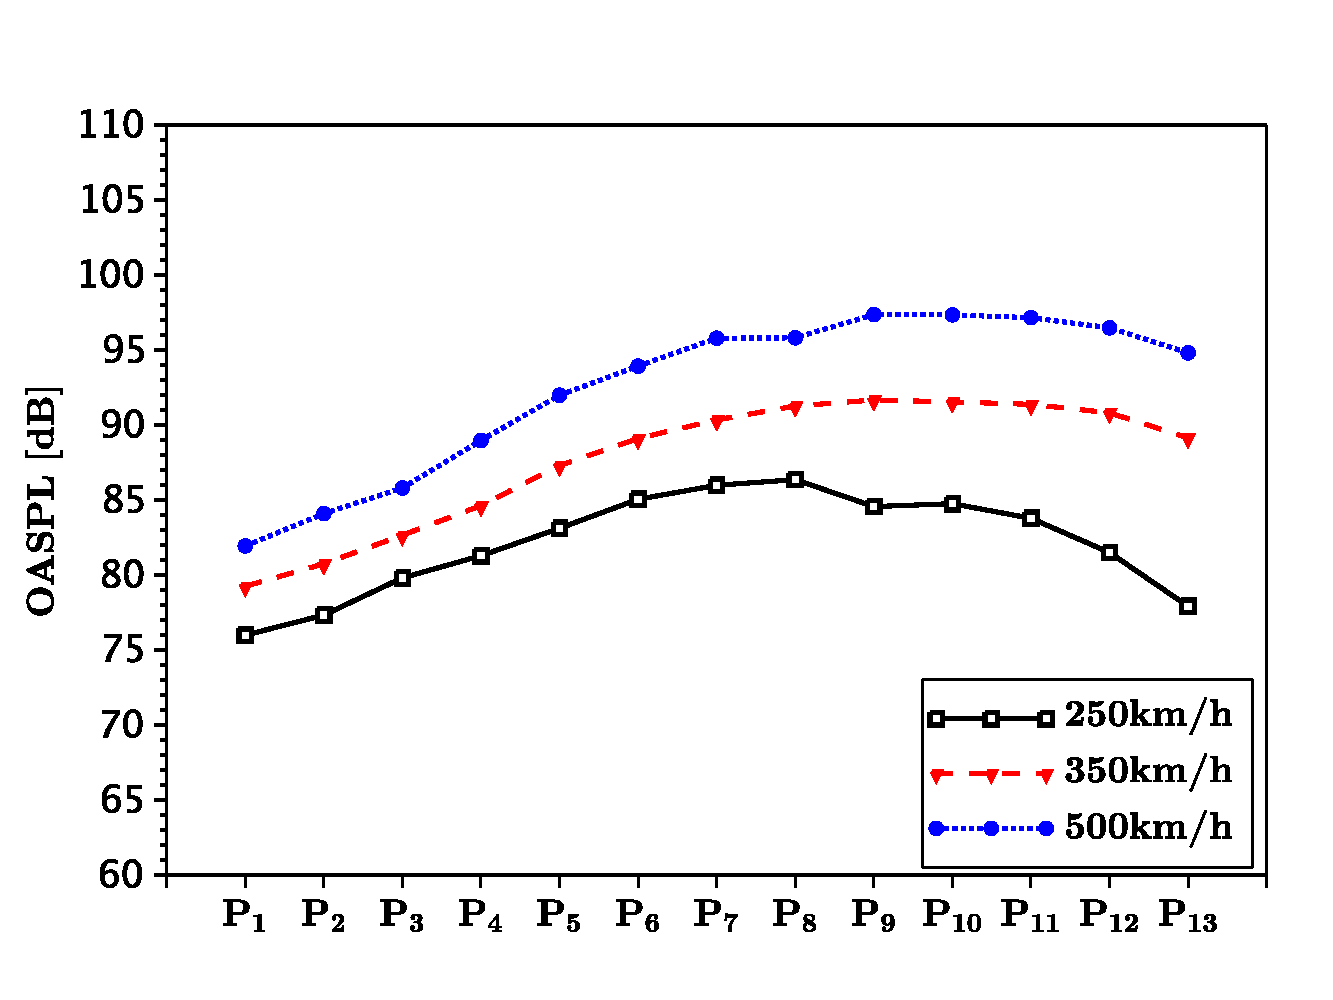
\includegraphics[width=\textwidth]{oaspl_c}
      \caption{}
      \label{fig:oaspl_c}
    \end{subfigure}%
    ~% add desired spacing
    \begin{subfigure}[b]{0.35\textwidth}
      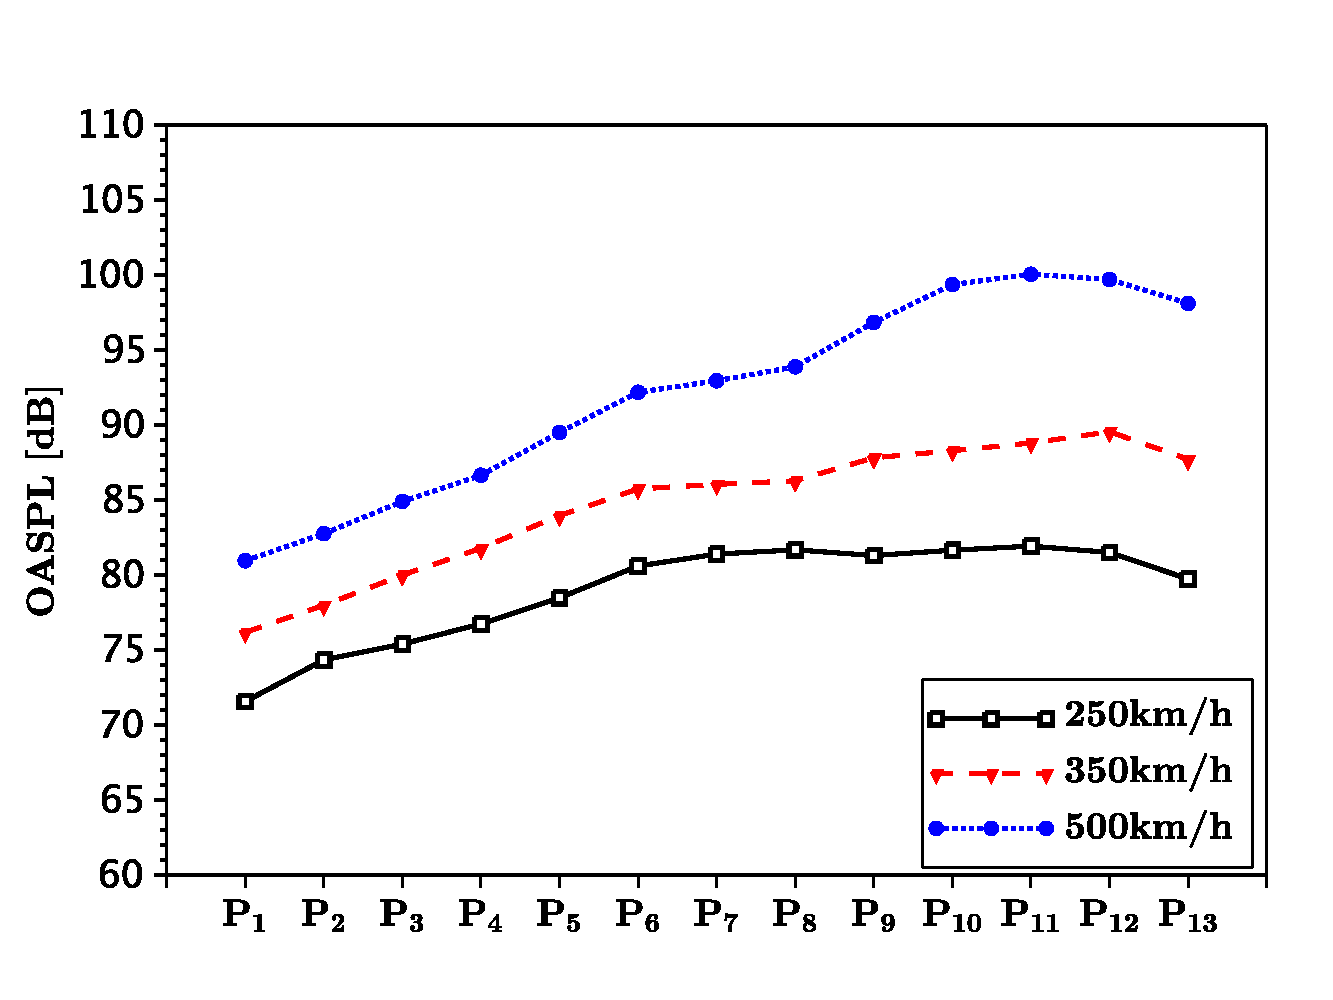
\includegraphics[width=\textwidth]{oaspl_d}
      \caption{}
      \label{fig:oaspl_d}
    \end{subfigure}
    \bicaption{\quad 多子图测试}{\quad A test for multi-subfig}
    \label{fig:oaspl}
\end{figure}

\subsection{表}

请见表~\ref{tab:sample}。
\begin{table}[!htbp]
    \bicaption{\quad 这是一个样表}{\quad This is a sample table}
    \label{tab:sample}
    \centering
    \footnotesize% fontsize
    \setlength{\tabcolsep}{4pt}% column separation
    \renewcommand{\arraystretch}{1.2}%row space 
    \begin{tabular}{lcccccccc}
        \hline
        行号 & \multicolumn{8}{c}{跨多列的标题}\\
        %\cline{2-9}% partial hline from column i to column j
        \hline
        Row 1 & $1$ & $2$ & $3$ & $4$ & $5$ & $6$ & $7$ & $8$\\
        Row 2 & $1$ & $2$ & $3$ & $4$ & $5$ & $6$ & $7$ & $8$\\
        Row 3 & $1$ & $2$ & $3$ & $4$ & $5$ & $6$ & $7$ & $8$\\
        Row 4 & $1$ & $2$ & $3$ & $4$ & $5$ & $6$ & $7$ & $8$\\
        \hline
    \end{tabular}
\end{table}

制图制表的更多范例,请见 \href{https://github.com/mohuangrui/ucasthesis/wiki}{ucasthesis 知识小站} 和 \href{https://en.wikibooks.org/wiki/LaTeX/Tables}{WiKibook Tables}。

\subsection{参考文献引用}

参考文献引用过程以实例进行介绍,假设需要引用名为"Document Preparation System"的文献,步骤如下:

1)将Bib格式的参考文献信息添加到ref.bib文件中(此文件位于Biblio文件夹下),如直接粘贴自网站,请注意修改其格式。

2)索引第一行 \verb|@article{lamport1986document,|中 \verb|lamport1986document| 即为此文献的label (中文文献也必须使用英文label,一般遵照:姓氏拼音+年份+标题第一字拼音的格式),想要在论文中索引此文献,\verb|\citep{lamport1986document}|。如此处所示 \textsuperscript{\citep{lamport1986document}}。

多文献索引用英文逗号隔开, 如此处所示 \textsuperscript{\citep{lamport1986document, chu2004tushu, chen2005zhulu}}。

更多例子如:

Walls等\textsuperscript{\citep{walls2013drought}}根据Betts\textsuperscript{\citep{betts2005aging}} 的研究,首次提出......理论。其中关于......的研究\textsuperscript{\citepns{walls2013drought, betts2005aging}},是当前中国得到迅速发展的研究领域 \textsuperscript{\citep{chen1980zhongguo, bravo1990comparative}}。

不同文献样式和引用样式,如著者-出版年制(authoryear)、顺序编码制(numbers)、上标顺序编码制(super)可在Thesis.tex中对artratex.sty调用实现,详见 \href{https://github.com/mohuangrui/ucasthesis/wiki}{ucasthesis 知识小站之文献样式}。

%若在上标顺序编码制(super)模式下,希望在特定位置将上标改为嵌入式标,可使用 \citetns{niu2013zonghe,stamerjohanns2009mathml} 和 \citepns{niu2013zonghe,stamerjohanns2009mathml}。

参考文献索引的更多知识,请见 \href{https://en.wikibooks.org/wiki/LaTeX/Bibliography_Management}{WiKibook Bibliography}。\nocite{*}% 使文献列表显示所有参考文献(包括未引用文献)

\section{常见使用问题}\label{sec:qa}

设置文档样式: 在artratex.sty中搜索关键字定位相应命令,然后修改
\begin{enumerate}
    \item 正文行距:启用和设置 \verb|\linespread{1.25}|,默认1.25倍行距。
    \item 参考文献行距:修改 \verb|\setlength{\bibsep}{0.0ex}|
    \item 目录显示级数:修改 \verb|\setcounter{tocdepth}{2}|
    \item 文档超链接的颜色及其显示:修改 \verb|\hypersetup|
\end{enumerate}

文档内字体切换方法:
    \begin{itemize}
        \item 宋体:国科大论文模板ucasthesis 或 \textrm{国科大论文模板ucasthesis}
        \item 粗宋体:{\bfseries 国科大论文模板ucasthesis} 或 \textbf{国科大论文模板ucasthesis}
        \item 黑体:{\sffamily 国科大论文模板ucasthesis} 或 \textsf{国科大论文模板ucasthesis}
        \item 粗黑体:{\bfseries\sffamily 国科大论文模板ucasthesis} 或 \textsf{\bfseries 国科大论文模板ucasthesis}
        \item 仿宋:{\ttfamily 国科大论文模板ucasthesis} 或 \texttt{国科大论文模板ucasthesis}
        \item 粗仿宋:{\bfseries\ttfamily 国科大论文模板ucasthesis} 或 \texttt{\bfseries 国科大论文模板ucasthesis}
        \item 楷体:{\itshape 国科大论文模板ucasthesis} 或 \textit{国科大论文模板ucasthesis}
        \item 粗楷体:{\bfseries\itshape 国科大论文模板ucasthesis} 或 \textit{\bfseries 国科大论文模板ucasthesis}
    \end{itemize}

\let\cleardoublepage\relax
}
